\subsection{Breadth First Search}
\noindent Breadth First Search (BFS), as the name says, explores the search space in the increasing order of the depth and the costs of traveling from one state to another is assumed to be a positive number. Typically, this algorithm is often associated with the concept of stack and queue and pushing and popping from the stack.

\begin{figure}[H]
	\centering
	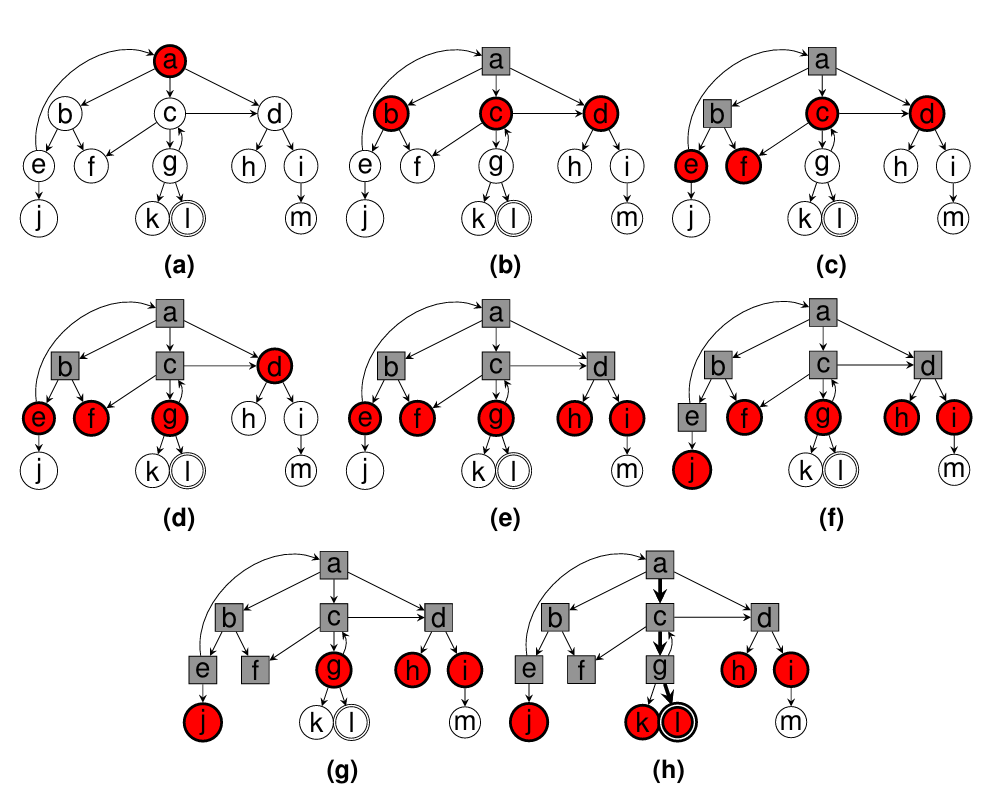
\includegraphics[width=0.8\textwidth]{./imgs/bfs.png}
	\caption{Breadth First Search (BFS)}
\end{figure}

\subsubsection{Pseudocode}
\begin{algorithm}[H]
	\caption{Breadth First Search (\textit{start, goal})}\label{alg:bfs}
	\begin{algorithmic}[1]
		\State queue \(gets\) [start]
		\While {queue is not empty}
		\State node \(gets\) dequeue(queue)
		\If {node = goal}
		\State return path
		\EndIf
		\ForAll {neighbor in valid moves}
		\If {neighbor not visited}
		\State mark neighbor as visited
		\State enqueue(queue, neighbor)
		\EndIf
		\EndFor
		\EndWhile
		\State return failure
	\end{algorithmic}
\end{algorithm}

\subsubsection{Implementation}

\subsubsection{Time and Space Complexity}
\textbf{Time Complexity:} \(O(V + E)\), where \(V\) is the number of vertices and \(E\) is the number of edges. Each node and edge is processed once.

\textbf{Space Complexity:} \(O(V)\) in the worst case, as the queue stores all nodes at the widest level of the graph.